\section{Results}\label{sec:results}

\subsection{Honest audits under coarse-graining}

The first empirical burden of the paper is methodological. If path-reversal asymmetry is to count as a directionality currency, then coarse observation must not manufacture it. We therefore evaluate the DPI-style margin
\[
\Delta=\SigmaT^{\mathrm{micro}}-\SigmaT^{\mathrm{coarse}}
\]
on pushed-forward trajectories across the frozen five-seed sweep described in Section~\ref{sec:methods}.

The result is clean. No violating seed-run survives the tolerance check, and the weakest aggregated audit margin remains positive. In the frozen summary, the minimum audit margin is \num{0.001069} (\code{min_delta_mean}). Figure~\ref{fig:results_dpi} shows the scan across the resolution ladder.

This matters conceptually as much as numerically. A putative directionality currency that can be created by forgetting variables would not be an honest audit of closure. The positive margin in the frozen sweep supports the stricter discipline adopted here: coarse observation may hide a directionality currency, but it does not create one from nothing, in line with the standard information-theoretic monotonicity intuition behind data-processing arguments \cite{coverthomas2006,kullback1951information}.

\begin{figure}[tbp]
    \centering
    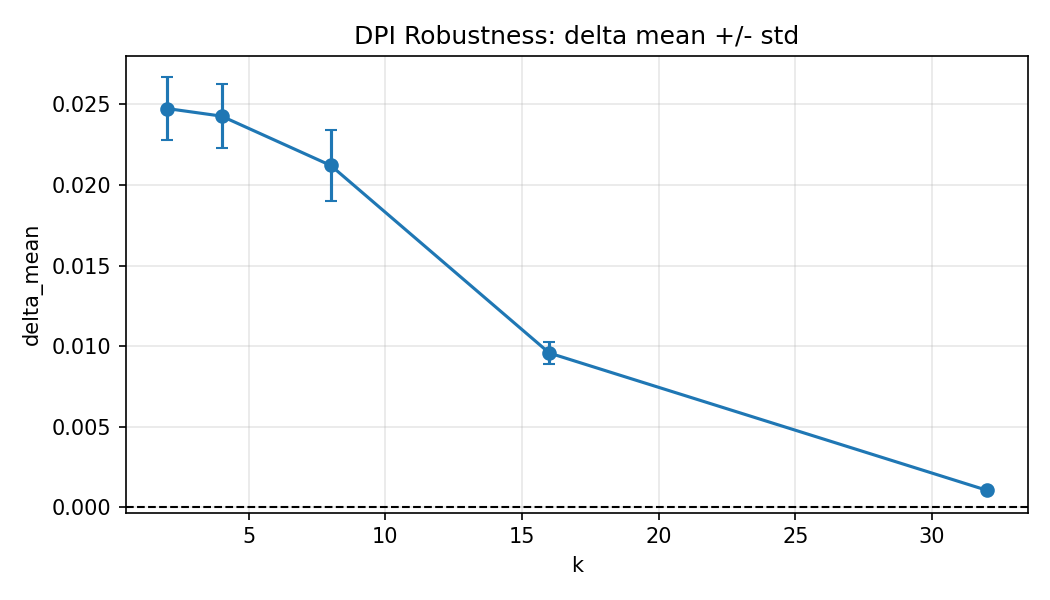
\includegraphics[width=0.88\linewidth,trim=0 0 0 25bp,clip]{figures/fig_dpi_scan.png}
    \caption{DPI-style audit honesty under coarse-graining. The plotted margin is \(\Delta=\SigmaT^{\mathrm{micro}}-\SigmaT^{\mathrm{coarse}}\) across the resolution ladder. Across the frozen five-seed sweep, no seed-run violates the tolerance check, and the minimum aggregated margin remains positive at \num{0.001069} (\code{min_delta_mean}).}
    \label{fig:results_dpi}
\end{figure}

\subsection{Price emergence and slack}

The second empirical burden is to show that shadow price is not an interpretive flourish but an induced coordinate of binding budget. Using the macro cost derived from lower-layer entropy-production-like increments, we sweep budgets and solve the single-constraint MaxCal closure from Section~\ref{sec:methods}. The aggregate monotonicity is nearly perfect: the frozen summary reports \num{-0.99923} for \code{spearman_rho_mean}.

Equally important, the same sweep exhibits a genuine slack regime. In every seed run, the high-budget tail contains a near-zero-price point; in the frozen summary, \code{n_tail_zero_lambda} is \(5\). Figure~\ref{fig:results_budget} shows the resulting price curve.

Together these two facts give the higher-layer interpretation of shadow price. When the lower-layer budget binds, \(\lambda\) is positive and reorganizes feasible transitions. When the budget is sufficiently relaxed, the dual currency collapses to zero. The price is therefore not an arbitrary fit parameter layered on top of the problem; it is the higher-layer response to an active lower-layer constraint.

\begin{figure}[tbp]
    \centering
    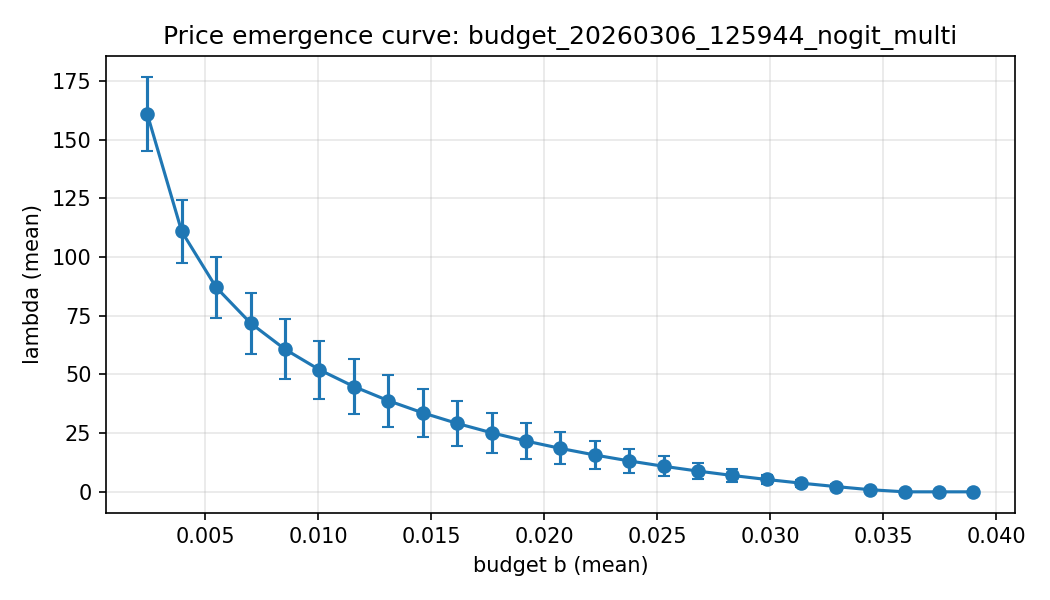
\includegraphics[width=0.88\linewidth,trim=0 0 0 25bp,clip]{figures/fig_budget_sweep.png}
    \caption{Shadow-price emergence from budget. The aggregated sweep shows a nearly perfect anti-monotone relation between budget and recovered price, with \code{spearman_rho_mean} = \num{-0.99923}. The high-budget tail enters the slack regime in every seed run, with \code{n_tail_zero_lambda} = \(5\).}
    \label{fig:results_budget}
\end{figure}

\subsection{Currency dimension grows with resolution}

The ladder experiment addresses a different part of the argument. If currencies are the low-dimensional coordinates in which a layer budgets or expresses drive, then finer resolution should reveal additional independent directions in which such currencies can live. We therefore summarize the visible loop structure of the coarse support graph by its cycle rank \(\betaone\) across the frozen coarse, intermediate, and fine lenses.

The frozen ladder summary reports \code{beta1_coarse_mean} = \(0\), \code{beta1_mid_mean} = \(5\), and \code{beta1_fine_mean} = \(11\). Figure~\ref{fig:results_ladder} shows the three-level increase.

This is the empirical version of a currency-dimension claim. At the coarsest level no independent loop survives, and thus no independent cycle-affinity coordinate is available. At intermediate and fine resolution, additional loop directions appear, enlarging the space in which distinct affinity currencies can in principle be expressed.

\begin{figure}[tbp]
    \centering
    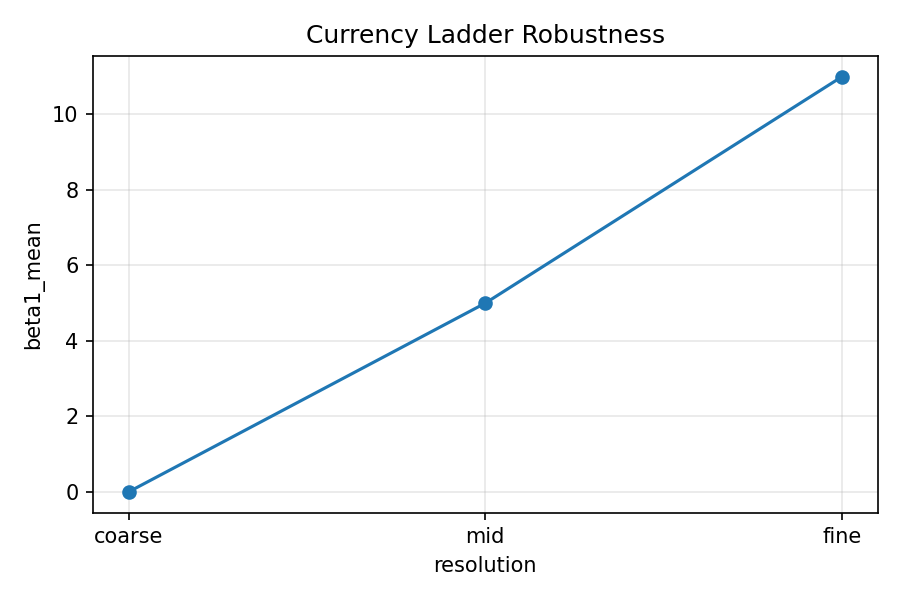
\includegraphics[width=0.88\linewidth,trim=0 0 0 25bp,clip]{figures/fig_currency_ladder.png}
    \caption{Resolution ladder and currency dimension. The frozen ladder summary reports \code{beta1_coarse_mean} = \(0\), \code{beta1_mid_mean} = \(5\), and \code{beta1_fine_mean} = \(11\). Finer resolution reveals more independent loop directions and therefore a larger space of potential cycle currencies.}
    \label{fig:results_ladder}
\end{figure}

\subsection{Proxy currencies fail}

The proxy-ablation experiment asks whether any low-dimensional penalty will do, or whether genuine currencies are structurally special. The answer is no. On held-out test data, the frozen summary reports \code{mean_nll_baseline} = \num{5.288}, \code{mean_nll_good} = \num{2.220}, and \code{mean_nll_bad} = \num{2.769}. The relative advantage of the structural cost over the proxy, measured on the baseline scale, is \num{0.1040} for \code{rel_adv}. Figure~\ref{fig:results_proxy} shows the comparison.

The same contrast appears in the stability of recovered prices. The frozen summary reports \code{std_lam_good} = \num{2.120} and \code{std_lam_bad} = \num{3.361}. The structurally aligned currency therefore does better on prediction and yields the more stable dual variable.

This is the strongest empirical reason for maintaining a strict definition of currency. A useful statistic can correlate with behavior without being the right spending coordinate of the layer. When the cost is structurally aligned with the lower-layer ledger, prediction improves and the inferred price stabilizes. When the cost is merely a proxy, both properties degrade.

\begin{figure}[tbp]
    \centering
    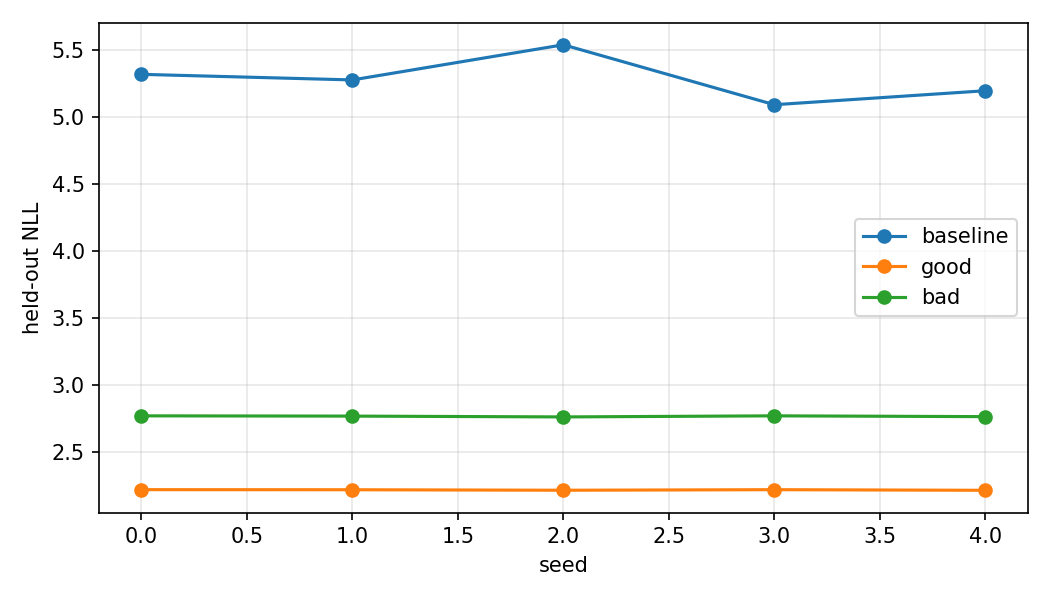
\includegraphics[width=0.88\linewidth]{figures/fig_proxy_ablation.png}
    \caption{Structural versus proxy currencies. Held-out performance favors the structurally aligned cost, with \code{mean_nll_good} = \num{2.220} versus \code{mean_nll_bad} = \num{2.769}, against \code{mean_nll_baseline} = \num{5.288}. The structural currency also yields the more stable recovered price, with \code{std_lam_good} = \num{2.120} versus \code{std_lam_bad} = \num{3.361}.}
    \label{fig:results_proxy}
\end{figure}

\subsection{Budgets buy object stability}

The last experiment closes the loop between budget and objecthood. Increasing maintenance price should not only change transition statistics; it should also make packaged objects more nearly idempotent under the packaging map. In the frozen summary, the relation between price and mean defect is essentially perfectly monotone, with \code{spearman_rho} numerically indistinguishable from \(-1\).

Across the sweep, mean defect falls from \code{defect_mean_max} = \num{0.1160} at the weakest enforcement end to \code{defect_mean_min} = \num{0.001443} at the strongest enforcement end. Figure~\ref{fig:results_idempotence} shows the defect-versus-price curve.

This is the most direct object-level signature in the paper. Budgets do not merely trade off motion against expenditure; they purchase closure coherence. Stronger enforcement makes packaged representatives more nearly fixed under package--evolve--repackage, which is exactly what the idempotence defect is designed to measure.

\begin{figure}[tbp]
    \centering
    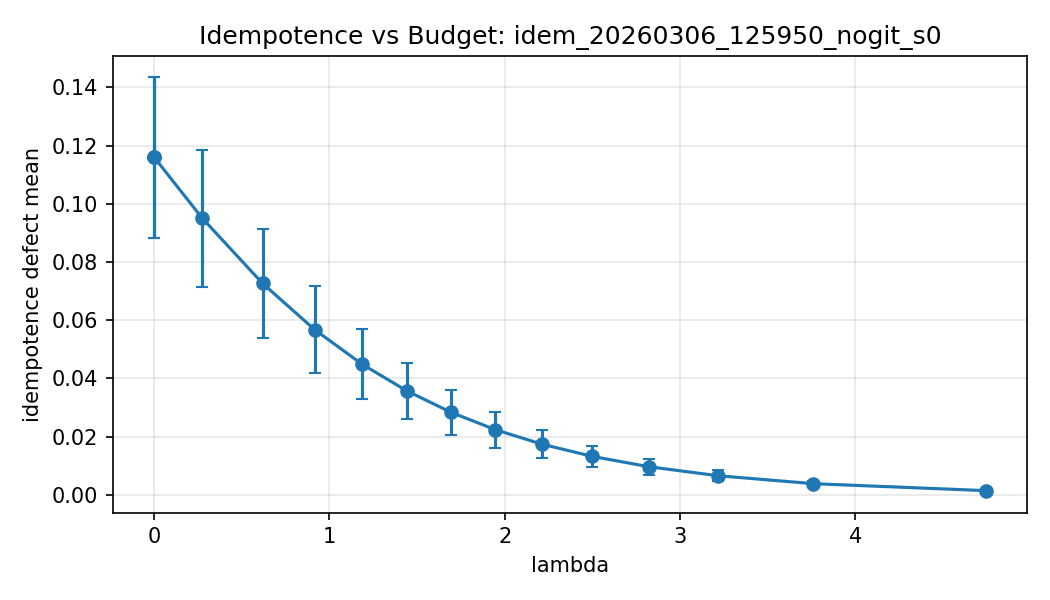
\includegraphics[width=0.88\linewidth,trim=0 0 0 25bp,clip]{figures/fig_idempotence_budget.png}
    \caption{Budgets buy object stability. The frozen idempotence summary reports \code{spearman_rho} numerically indistinguishable from \(-1\) between price and mean defect. Across the sweep, mean defect drops from \code{defect_mean_max} = \num{0.1160} to \code{defect_mean_min} = \num{0.001443}.}
    \label{fig:results_idempotence}
\end{figure}

\FloatBarrier
